
    \documentclass[tikz,convert={outfile=\jobname.png}]{standalone}
    \usetikzlibrary{mindmap,trees,backgrounds}
    \usepackage{fontspec}
    \defaultfontfeatures{Ligatures=TeX,Scale=3}
    \setmainfont{M+ 1mn}
    
    
    \definecolor{light blue}{RGB}{166, 206, 227}
    \definecolor{dark blue}{RGB}{31, 120, 180}
    \definecolor{light green}{RGB}{178, 223, 138}
    \definecolor{dark green}{RGB}{51, 160, 44}
    \definecolor{pink}{RGB}{251, 154, 153}
    \definecolor{red}{RGB}{227, 26, 28}
    \definecolor{beige}{RGB}{253, 191, 111}
    \definecolor{black}{RGB}{0.0, 0.0, 0.0}
    \definecolor{darkgray}{RGB}{168.3, 168.3, 168.3}
    \definecolor{white}{RGB}{255.0, 255.0, 255.0}
    
    \begin{document}
    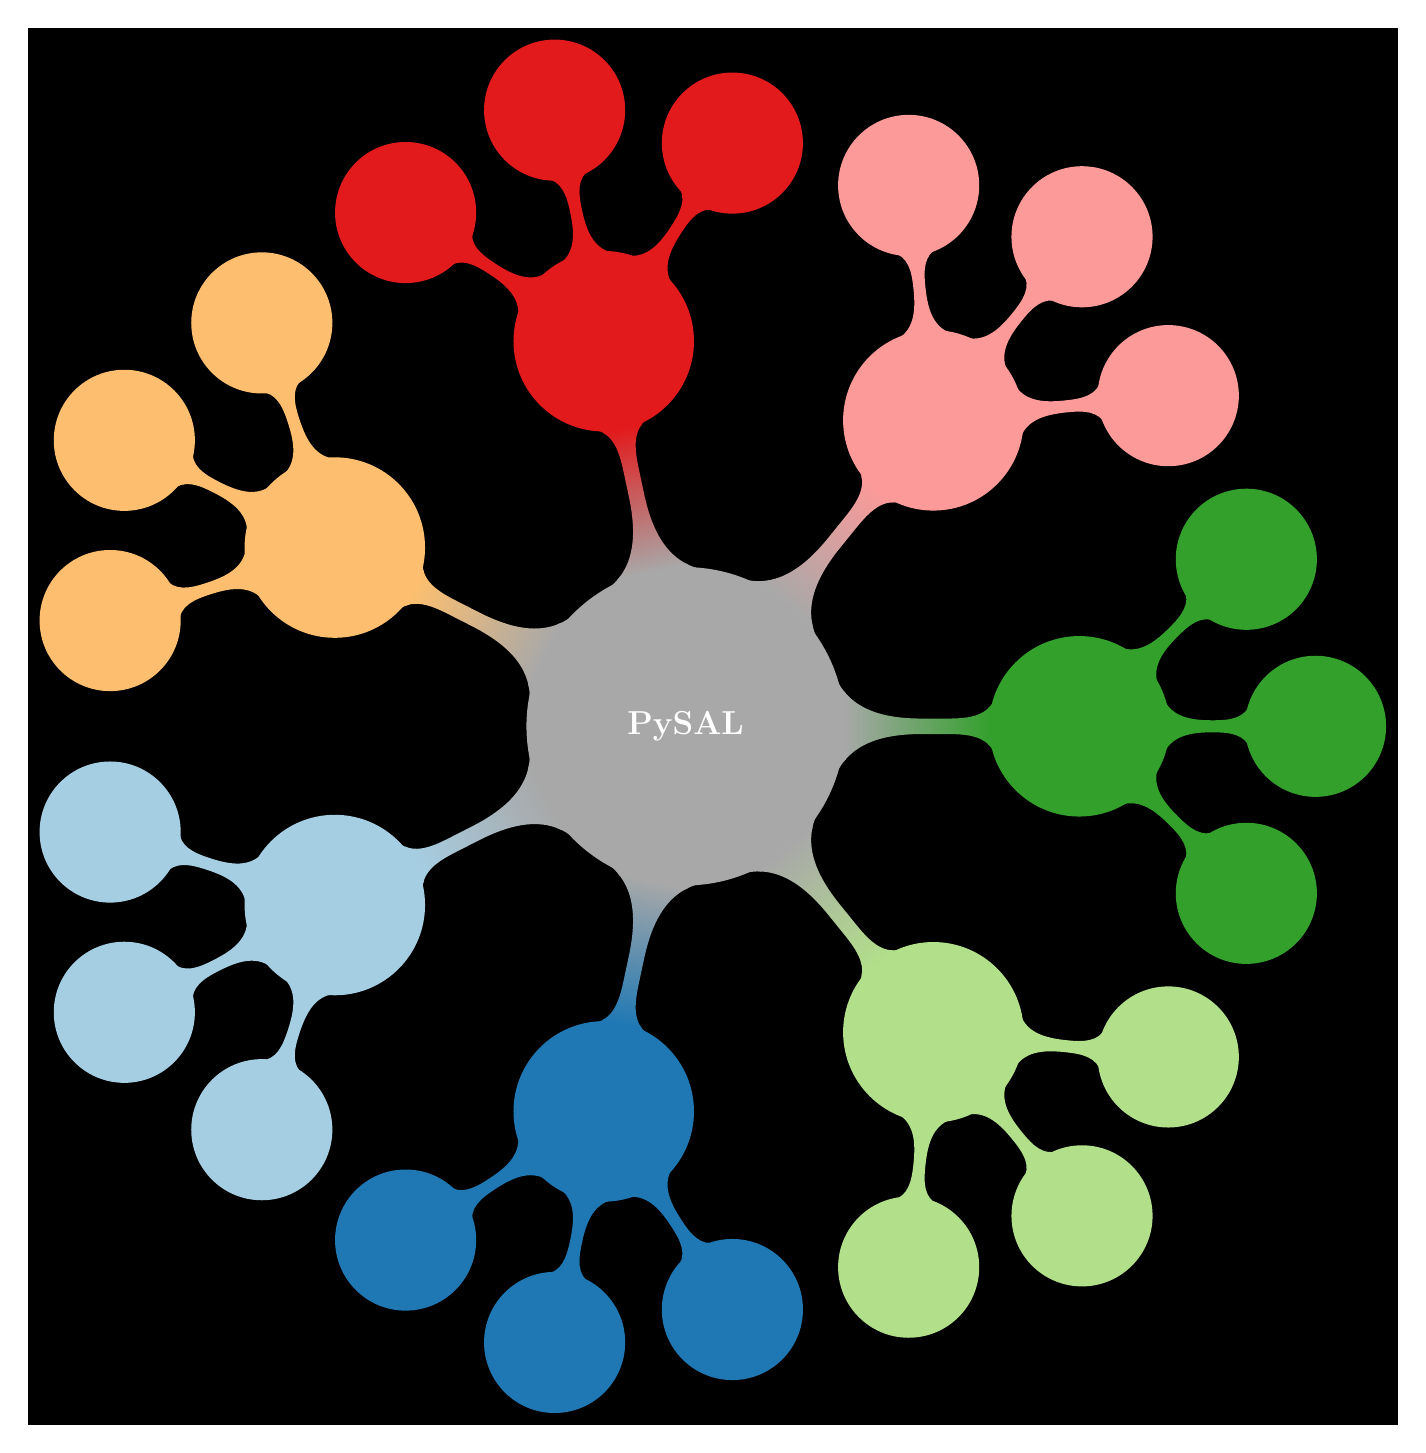
\begin{tikzpicture}[
        background rectangle/.style={fill=black},
        show background rectangle,
        mindmap,
        grow cyclic,
        every node/.style=concept,
        concept color=darkgray,
        text=white,
        level 1/.append style={
            level distance=5cm,
            sibling angle=51,
            font=\Huge
        },
        level 2/.append style={
            level distance=3cm,
            sibling angle=45
        }
    ]
    
        \node[concept color=darkgray]{\large\bfseries{PySAL}}
        child [concept color=light blue]{ node {}
            child { node { }}
            child { node { }}
            child { node { }}
         }
        child [concept color=dark blue]{ node {}
            child { node { }}
            child { node { }}
            child { node { }}
         }
        child [concept color=light green]{ node {}
            child { node { }}
            child { node { }}
            child { node { }}
         }
        child [concept color=dark green]{ node {}
            child { node { }}
            child { node { }}
            child { node { }}
         }
        child [concept color=pink]{ node {}
            child { node { }}
            child { node { }}
            child { node { }}
         }
        child [concept color=red]{ node {}
            child { node { }}
            child { node { }}
            child { node { }}
         }
        child [concept color=beige]{ node {}
            child { node { }}
            child { node { }}
            child { node { }}
         }
                ;
    \end{tikzpicture}
    \end{document}